
% This LaTeX was auto-generated from MATLAB code.
% To make changes, update the MATLAB code and republish this document.

\documentclass{article}
\usepackage{graphicx}
\usepackage{color}

\sloppy
\definecolor{lightgray}{gray}{0.5}
\setlength{\parindent}{0pt}

\begin{document}

    
    \begin{verbatim}
clc
clear
close all
oo = zeros(1000,1);
ono = ones(1000,1);
omo = linspace(0,1,1000)';
oro = linspace(1,0,1000)';

RSrun_states_estim(:,3) = [oo;omo;ono;oro];
RSrun_states_estim(:,2) = [omo;ono;oro;oo];
plot(RSrun_states_estim(:,3),RSrun_states_estim(:,2));
hold all;
plot(RSrun_states_estim(1,3),RSrun_states_estim(1,2),'rx');
plot(RSrun_states_estim(end,3),RSrun_states_estim(end,2),'gx');
%plot(RSrun_posVIS(visUpdatesAvlble,3),RSrun_posVIS(visUpdatesAvlble,2),'o-');
%set(gca,'xaxisLocation','top')
%set(gca,'Xdir','reverse')
legend({'$\hat{Pos}$','start','finish','$\hat{Pos}_{VIS}$'},'Location','best','Interpreter', 'latex')
%ylim([-.3 .3]);
title('Reference Input Trajectory')
xlabel({'$X$ [m]'},'Interpreter','latex');
ylabel({'$Y$ [m]'},'Interpreter','latex');
xlim([-.2,1.5])
axis equal
\end{verbatim}

        \color{lightgray} \begin{verbatim}Warning: Ignoring extra legend entries. 
\end{verbatim} \color{black}
    
\includegraphics [width=4in]{fake_01.eps}



\end{document}
    
